	\makeatletter
	\def\@makechapterhead#1{%
	  \vspace*{50\p@}%
	  {\parindent \z@ \centering\normalfont
	    \ifnum \c@secnumdepth >\m@ne
	      \if@mainmatter
	         \Large\bfseries \@chapapp\space \thechapter
 	        \par\nobreak
	        \vskip 20\p@
	      \fi
	    \fi
	    \interlinepenalty\@M
	     \Large \bfseries #1\par\nobreak
	
	    \vskip 40\p@
	  }}
	\def\@makeschapterhead#1{%
	  \vspace*{50\p@}%
	  {\parindent \z@ \centering 
	    \normalfont
	    \interlinepenalty\@M
	    \Large\bfseries  #1\par\nobreak
	    \vskip 40\p@
	  }}
	\makeatother
	\titlespacing*{\chapter}{0pt}{0pt}{12pt}

\chapter{Modules}


\section{Module Description}
The modules functionality has been defined below with the snippets code

\subsection{Splash Startup}

A splash screen is an image that appears while a game or program is loading. It may also be used to describe an introduction page on a website. Splash screens cover the entire screen or simply a rectangle near the center of the screen. The splash screens of operating systems and some applications that expect to be run full-screen usually cover the entire screen.

Splash screens are typically used by particularly large applications to notify the user that the program is in the process of loading. They provide feedback that a lengthy process is underway. Occasionally, a progress bar within the splash screen indicates the loading progress. A splash screen disappears when the application's main window appears.
Splash screens typically serve to enhance the look and feel of an application or web site, hence they are often visually appealing. They may also have animations, graphics, and sound.

The Java programming language has a specific class for creating splash screens,  that handles standard splash screen functions, e.g. display an image centered on screen then disappears when the first program window opens.
Type the Code and Few lines here



\subsection{Async Task }

AsyncTask enables proper and easy use of the UI thread. This class allows to perform background operations and publish results on the UI thread without having to manipulate threads and/or handlers.

AsyncTask is designed to be a helper class around Thread and Handler and does not constitute a generic threading framework. AsyncTasks should ideally be used for short operations (a few seconds at the most.) If you need to keep threads running for long periods of time, it is highly recommended you use the various APIs provided by the java.util.concurrent pacakge such as Executor, ThreadPoolExecutor and FutureTask.

An asynchronous task is defined by a computation that runs on a background thread and whose result is published on the UI thread. An asynchronous task is defined by 3 generic types, called Params, Progress and Result, and 4 steps, called onPreExecute, doInBackground, onProgressUpdate and onPostExecute.

\lstinputlisting{async.py}

\subsection{JSON parser}

JSON (JavaScript Object Notation) is a lightweight data-interchange format. It is easy for humans to read and write.

 It is easy for machines to parse and generate. It is based on a subset of the JavaScript Programming Language, Standard ECMA-262 3rd Edition - December 1999. JSON is a text format that is completely language independent but uses conventions that are familiar to programmers of the C-family of languages, including C, C++, C#, Java, JavaScript, Perl, Python, and many others. These properties make JSON an ideal data-interchange language.

JSON is built on two structures:

\begin{description}
 \item[$\bullet$ ]  A collection of name/value pairs. In various languages, this is realized as an object, record, struct, dictionary, hash  table, keyed list, or associative array.
 \item[$\bullet$ ]  An ordered list of values. In most languages, this is realized as an array, vector, list, or sequence.

These are universal data structures. Virtually all modern programming languages support them in one form or another. It makes sense that a data format that is interchangeable with programming languages also be based on these structures.



\lstinputlisting{json.txt}

\end{description}
\subsection{SQL Lite Helper}
A helper class to manage database creation and version management.You create a subclass implementing onCreate (SQLiteDatabase), onOpen (SQLiteDatabase), and this class takes care of opening the database if it exists, creating it if it does not, and upgrading it as necessary. Transactions are used to make sure the database is always in a sensible state.This class makes it easy for ContentProvider implementations to defer opening and upgrading the database until first use, to avoid blocking application startup with long-running database upgrades.Exposes methods to manage a SQLite database.SQLiteDatabase has methods to create, delete, execute SQL commands, and perform other common database management tasks.See the Notepad sample application in the SDK for an example of creating and managing a database.Database names must be unique within an application, not across all applications
\lstinputlisting{sqllitehelper.py}

\subsection{GPS Receiver}

Android gives your applications access to the location services supported by the device through classes in the android.location package. The central component of the location framework is the LocationManager system service, which provides APIs to determine location and bearing of the underlying device (if available).As with other system services, you do not instantiate a LocationManager directly. Rather, you request an instance from the system by calling LOCATION_SERVICE.


\lstinputlisting{gps.py}


\subsection{Google Maps API}
With the Google Maps Android API, you can add maps to your app that are based on Google Maps data. The API automatically handles access to Google Maps servers, data downloading, map display, and touch gestures on the map. You can also use API calls to add markers, polygons and overlays, and to change the user's view of a particular map area.

The key class in the Google Maps Android API is MapView. A MapView displays a map with data obtained from the Google Maps service. When the MapView has focus, it will capture keypresses and touch gestures to pan and zoom the map automatically,including handling network requests for additional maps tiles. It also provides all of the UI elements necessary for users to control the map. Your application can also use MapView class methods to control the map programmatically and draw a number of overlays on top of the map.

The Google Maps Android APIs are not included in the Android platform, but are available on any device with the Google Play Store running Android 2.2 or higher, through Google Play services.
To integrate Google Maps into your app, you need to install the Google Play services libraries for your Android SDK..
%\begin{figure} [ht]
%\centering
%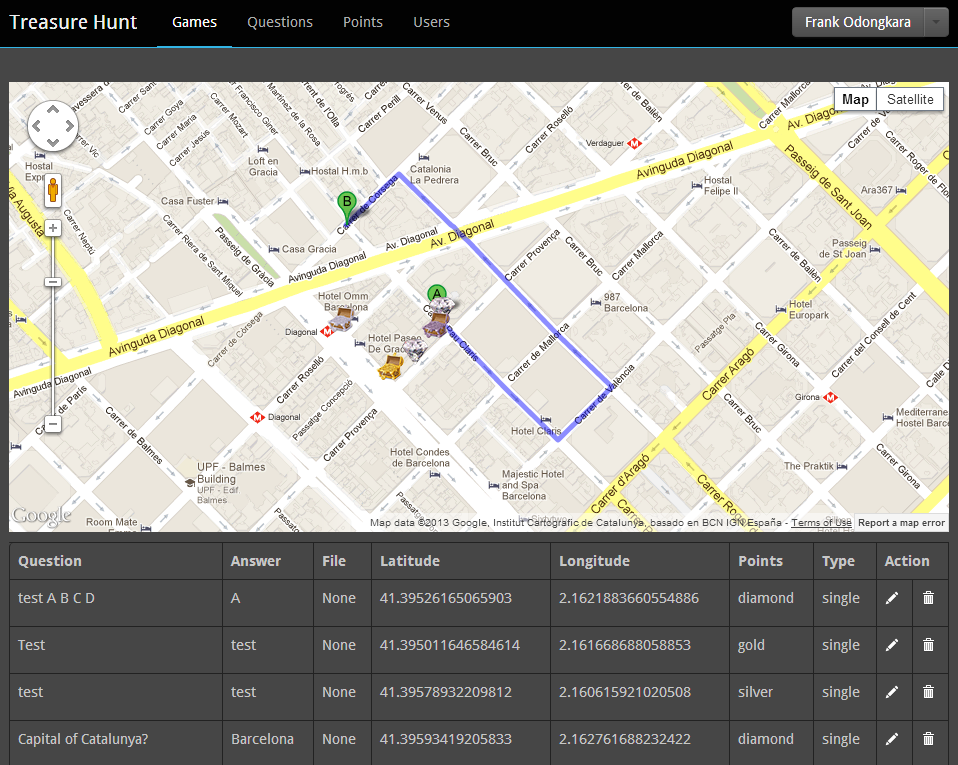
\includegraphics[scale=0.5]{images/maps}\\
%\caption{Custom Maps Designed }
%\label{Game Master Designs the Game with this Map}
%\end{figure}








